\chapter{Process Automation}

After doing a domain analysis, we will execute the process. 

\begin{enumerate}
    \item Create an executable BPMN model in Camunda Modeler. 
    \item Create a functional application that supports the BPMN model using the Camunda BPM.
    \item Create forms for BPMN activities. 
    \item Execute the BPMN model. One happy flow, one unhappy flow. 
    \item Create one meaningful report in the Analytics section
    \item Demonstrate your results in a presentation. See~\cref{sec:presentation}. 
\end{enumerate}

\section{Process Design}

Insert the process models in BPMN and DMN. 

\begin{landscape}
    \begin{figure}[h]\centering
        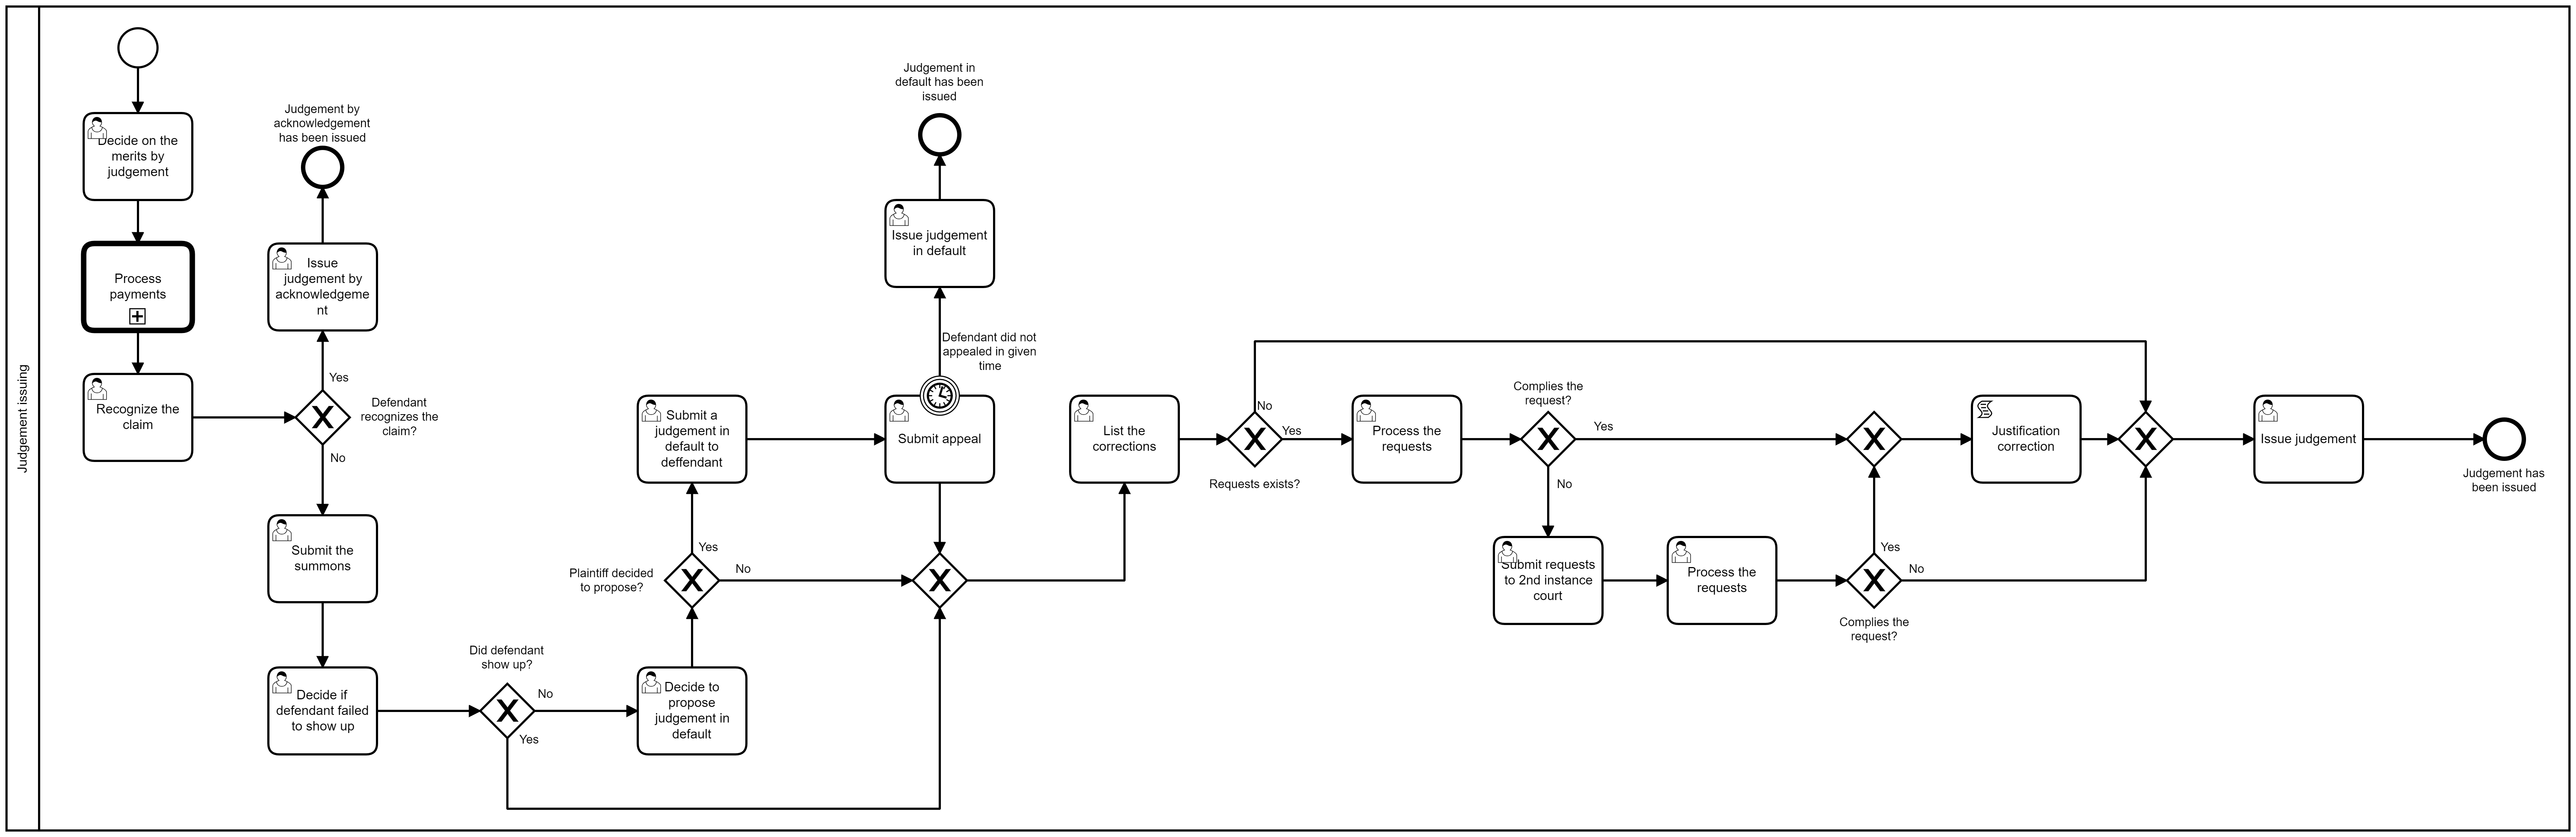
\includegraphics[width=\textwidth]{pic/bpmn}
        \caption{BPMN diagram}
        \label{fig:bpmnModel}
    \end{figure}
\end{landscape}

\section{Process Execution}

Include screenshots of all the important execution steps here. 

\section{Results Presentation}\label{sec:presentation}

An url to your 2 min presentation where you present an executive level summary of your efforts. Imagine you are presenting it to a customer who paid 100k EUR for the work. \url{https://www.youtube.com/watch?v=qfprck_Djro} 